\documentclass[UTF8]{article}
\usepackage{graphicx}
\usepackage{subfigure}
\usepackage{amsmath}
\usepackage{makecell}
\usepackage[utf8]{inputenc}
\usepackage[space]{ctex} %中文包
\usepackage{listings} %放代码
\usepackage{xcolor} %代码着色宏包
\usepackage{CJK} %显示中文宏包
\usepackage{float}
\usepackage{makecell}
\usepackage{diagbox}
\usepackage{bm}
\usepackage{ulem} 
\usepackage{amssymb}
\usepackage{soul}
\usepackage{color}
\usepackage{geometry}
\usepackage{fancybox} %花里胡哨的盒子
\usepackage{xhfill} %填充包, 可画分割线 https://www.latexstudio.net/archives/8245
\usepackage{multicol} %多栏包
\usepackage{enumerate} %可以方便地自定义枚举标题
\usepackage{multirow} %表格中多行单元格合并
\usepackage{wasysym} %可以使用wasysym里的一堆奇奇怪怪的符号
%\usepackage{mips}

\geometry{left = 2.5cm, right = 2.5cm, bottom = 2.5cm, top = 3cm}

\definecolor{mygreen}{rgb}{0,0.6,0}
\definecolor{mygray}{rgb}{0.5,0.5,0.5}
\definecolor{mymauve}{rgb}{0.58,0,0.82}

\lstset{
	backgroundcolor=\color{white}, 
	%\tiny < \scriptsize < \footnotesize < \small < \normalsize < \large < \Large < \LARGE < \huge < \Huge
	basicstyle = \scriptsize,       
	breakatwhitespace = false,        
	breaklines = true,                 
	captionpos = b,                    
	commentstyle = \color{mygreen}\bfseries,
	escapeinside=``,
	extendedchars = false,
	frame = shadowbox, 
	framerule=0.5pt,
	keepspaces=true,
	keywordstyle=\color{blue}\bfseries, % keyword style
	language = verilog,                     % the language of code
	otherkeywords={string}, 
	numbers=left, 
	numbersep=5pt,
	numberstyle=\tiny\color{mygray},
	rulecolor=\color{black},         
	showspaces=false,  
	showstringspaces=false, 
	showtabs=false,    
	stepnumber=1,         
	stringstyle=\color{mymauve},        % string literal style
	tabsize=4,          
	title=\lstname,
	texcl=true  
}

%\sum\nolimits_{j=1}^{M}   上下标位于求和符号的水平右端,
%\sum\limits_{j=1}^{M}   上下标位于求和符号的上下处,
%\sum_{j=1}^{M}  对上下标位置没有设定,会随公式所处环境自动调整。

%%%%%%%%%%%%%画图包%%%%%%%%%%%%%
\usepackage{tikz}
%%%%%%%%%%%%%画图背景包%%%%%%%%%%%%%
\usetikzlibrary{backgrounds}

%%%%%%%%%%%%%在tikz中画一个顶点%%%%%%%%%%%%%
%%%%%%%%%%%%%#1:node名称%%%%%%%%%%%%%
%%%%%%%%%%%%%#2:位置%%%%%%%%%%%%%
%%%%%%%%%%%%%#3:标签%%%%%%%%%%%%%
\newcommand{\newVertex}[3]{\node[circle, draw=black, line width=1pt, scale=0.8] (#1) at #2{#3}}
%%%%%%%%%%%%%在tikz中画一条边%%%%%%%%%%%%%
\newcommand{\newEdge}[2]{\draw [black,very thick](#1)--(#2)}
%%%%%%%%%%%%%在tikz中放一个标签%%%%%%%%%%%%%
%%%%%%%%%%%%%#1:名称%%%%%%%%%%%%%
%%%%%%%%%%%%%#2:位置%%%%%%%%%%%%%
%%%%%%%%%%%%%#3:标签内容%%%%%%%%%%%%%
\newcommand{\newLabel}[3]{\node[line width=1pt] (#1) at #2{#3}}

%%%%%%%%%%%%%强制跳过一行%%%%%%%%%%%%%
\newcommand{\jumpLine} {\hspace*{\fill} \par}
%%%%%%%%%%%%%关键点指令,可用itemise替代%%%%%%%%%%%%%
\newcommand{\average}[1]{\left\langle #1\right\rangle }
%%%%%%%%%%%%%表格内嵌套表格%%%%%%%%%%%%%

\newcommand{\keypoint}[2]{$\bullet$\textbf{#1}\quad#2\par}
%%%%%%%%%%%%%<T>平均值表示%%%%%%%%%%%%%
\newcommand{\tabincell}[2]{\begin{tabular}{@{}#1@{}}#2\end{tabular}}%放在导言区
%%%%%%%%%%%%%大黑点item头%%%%%%%%%%%%%
\newcommand{\itemblt}{\item[$\bullet$]}
%%%%%%%%%%%%%大圈item头%%%%%%%%%%%%%
\newcommand{\itemc}{\item[$\circ$]}
%%%%%%%%%%%%%大星星item头%%%%%%%%%%%%%
\newcommand{\itembs}{\item[$\bigstar$]}
%%%%%%%%%%%%%右▷item头%%%%%%%%%%%%%
\newcommand{\itemrhd}{\item[$\rhd$]}
%%%%%%%%%%%%%定义为%%%%%%%%%%%%%
\newcommand{\defas}{=_{df}}
%%%%%%%%%%%%%蕴含%%%%%%%%%%%%%
\newcommand{\imp}{\rightarrow}

%%%%%%%%%%%%%双线分割线%%%%%%%%%%%%%
\newcommand*{\doublerule}{\hrule width \hsize height 1pt \kern 0.5mm \hrule width \hsize height 2pt}
%%%%%%%%%%%%%双线中间可加东西的分割线%%%%%%%%%%%%%
\newcommand\doublerulefill{\leavevmode\leaders\vbox{\hrule width .1pt\kern1pt\hrule}\hfill\kern0pt }
%%%%%%%%%%%%%左大括号%%%%%%%%%%%%%
\newcommand{\leftbig}[1]{\left\{\begin{array}{l}#1\end{array}\right.}
%%%%%%%%%%%%%矩阵%%%%%%%%%%%%%
\newcommand{\mat}[2]{\left[\begin{array}{#1}#2\end{array}\right]}
%%%%%%%%%%%%%可换行圆角文本框%%%%%%%%%%%%%
\newcommand{\ovalboxn}[1]{\ovalbox{\tabincell{l}{#1}}}
%%%%%%%%%%%%%设置section的counter, 使从0开始%%%%%%%%%%%%%
\setcounter{section}{0}

\title{计算机组成原理实验 实验报告}
\date{}

\begin{document}
%%%%%%%%%%%%%科大报告封面%%%%%%%%%%%%%
\maketitle
\begin{figure}[H]
	\centering
	
\includegraphics[width=2.5in]{xiaohui.png}\vspace{0.5cm}\\
	\large{
		实验题目:Lab2 寄存器堆与队列\\
		学生姓名:王章瀚\\
		学生学号:PB18111697\\
		完成日期:\today\\
	}\vspace{2cm}
	
	\large{计算机实验教学中心制\\2019年09月\\}
	\thispagestyle{empty}
	\clearpage  % 清除当页页码
\end{figure}
\newpage

\section{实验题目}
Lab2 寄存器堆与队列

\section{实验目的}
\begin{enumerate}
	\item 掌握寄存器堆(Register File)和存储器(Memory)的功能、时序及其应用;
	\item 熟练掌握数据通路和控制器的设计和描述方法。
\end{enumerate}

\section{实验平台}
Vivado

\section{实验过程}
\subsection{寄存器堆}
这里寄存器堆的要求是: 该寄存器堆含有32 个寄存器(r0 ~ r31,其中r0的内容恒定为零), 寄存器的位宽由参数WIDTH指定, 具有2个异步读端口和1个同步写端口。
因此只需要维护一个这样的寄存器数组:\par
\begin{center}
	\ovalboxn{reg [WIDTH-1: 0] registers[SIZE-1: 0];}
\end{center}
然后在we使能的时候对寄存器进行相应修改, 并固定0地址输出为0即可. 代码相对简单, 直接贴上.
\begin{lstlisting}[language=verilog]
module register_file
    #(
    parameter WIDTH = 32,   // 数据宽度
    parameter ADDR_WIDTH = 5, // 地址长度
    parameter SIZE = {1'b1, {(ADDR_WIDTH){1'b0}}} // 地址数量
    )
    (
    input clk,    // 时钟(上升沿有效)
    input [ADDR_WIDTH-1: 0] ra0,   // 读端口0地址
    output [WIDTH-1: 0] rd0,    //读端口0数据
    input [ADDR_WIDTH-1: 0] ra1,   // 读端口1地址
    output [WIDTH-1: 0] rd1,    //读端口1数据
    input [ADDR_WIDTH-1: 0] wa,  // 写端口位置
    input we,   // 写使能(高电平有效)
    input [WIDTH-1: 0] wd   // 写端口数据
    );
    
    reg [WIDTH-1: 0] registers[SIZE-1: 0];
    
    assign rd0 = ra0 == {ADDR_WIDTH{1'b0}} ? {WIDTH{1'b0}} : registers[ra0]; // 保证了0地址输出为0
    assign rd1 = ra1 == {ADDR_WIDTH{1'b0}} ? {WIDTH{1'b0}} : registers[ra1]; // 保证了0地址输出为0
    
    always @(posedge clk) begin
        if(we) begin
            if(wa != {ADDR_WIDTH{1'b0}}) begin
                registers[wa] <= wd;
            end
        end
    end
    
endmodule
\end{lstlisting}
\subsection{存储器}
\subsubsection{行为方式描述存储器}
这里填补了老师留的空. 由于不是实验步骤要求的, 这里只是提一下.
\begin{lstlisting}[language=verilog]
module  ram_16x8			//16x8位单端口RAM
    (
    input  clk, 			//时钟(上升沿有效)
    input en, we,				//使能,写使能
    input [3: 0]  addr,	//地址
    input [7: 0]  din,		//输入数据
    output [7: 0]  dout	//输出数据
    );
    reg [3: 0] addr_reg;
    reg [7: 0] mem[15: 0];
    
    //初始化RAM的内容
    initial
    $readmemh("init.mem", mem); 
    
    assign dout = mem[addr_reg];
    
    always@(posedge clk) begin
        if(en) begin
            addr_reg <= addr;
            if(we)
                mem[addr] <= din;
        end
    end
endmodule
\end{lstlisting}
\subsubsection{IP核例化存储器}
\begin{enumerate}
	\item 分布式存储器(Distributed Memory Generator)\par
	修改相应 Depth 和 Data Width 等即可.
	\begin{figure}[H]
		\centering
		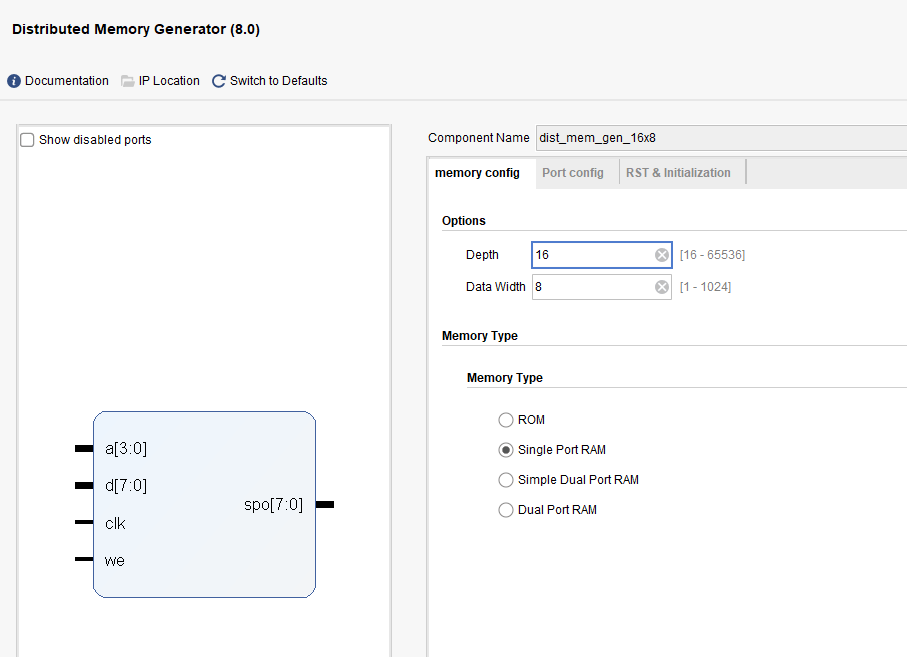
\includegraphics[scale=0.4]{IP_dist.png}
	\end{figure}\par
	
	\item 块式存储器(Block Memory Generator)\par
	修改相应 Write Width, Write Depth 和 Read Width, Read Depth 等即可.
	\begin{figure}[H]
		\centering
		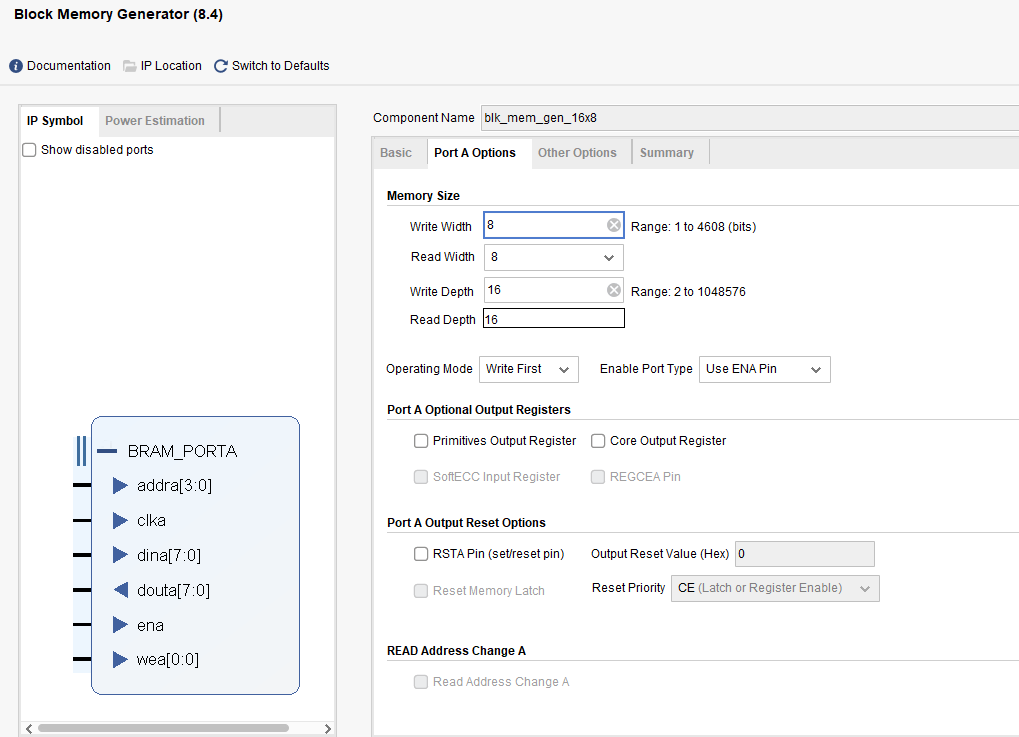
\includegraphics[scale=0.4]{IP_blk.png}
	\end{figure}\par
	
	\item 功能仿真结果与对比\par
	仿真结果见下图, dout\_dist和dout\_blk分别是分布式存储器和块式存储器的仿真输出结果.
	可见写的时候, 二者都是同步写入(图中标识了写ff到地址00上的时刻).
	而读的时候, 分布式存储器是异步读, 而块式的则是同步读(正是因此, 块式的输出结果总是落后一个周期).
	\begin{figure}[H]
		\centering
		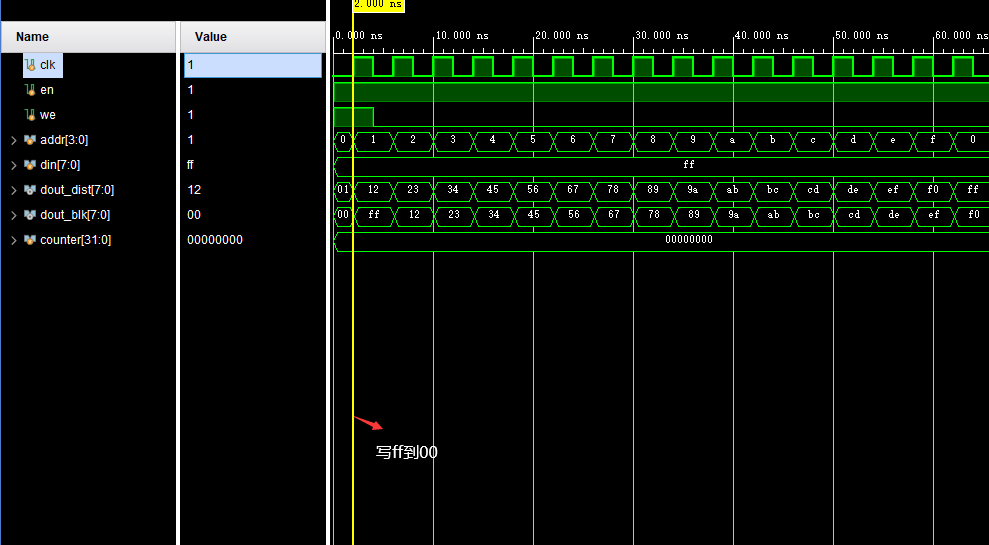
\includegraphics[scale=0.4]{difference_blk_dist.png}
	\end{figure}\par
	至于其他方面的对比, 大致可见下表
	\begin{center}
		\begin{tabular}{|c|c|c|}
		\hline
		 & 分布式存储器 & 块式存储器 \\
		\hline
		读的方式 & 异步 & 同步 \\
		\hline
		写的方式 & 同步 & 同步 \\
		\hline
		物理资源使用 & CLB的LUT & 独立的专门存储器 \\
		\hline
		适用情形 & 小存储器 & 大存储器 \\
		\hline
		\end{tabular}
	\end{center}
\end{enumerate}
\subsection{FIFO队列电路}
\subsubsection{基本过程}
这里采用一个小状态机来实现. 状态由两部分组成: head\_ptr(队列头指针)和tail\_ptr(队列尾指针). 然后每当有入队或出队的使能信号, 就准备好数据送入块式存储器, 待从块式存储器中取出数据之后, 就输出出来. 这其中, 对使能信号做了取边沿处理, 以防使能周期过长.
\subsubsection{数据通路}
这里数据通路较为复杂, 故直接用Vivado的RTL分析得到的结果来分析. 各个模块功能已经标注如下图
\begin{figure}[H]
	\centering
	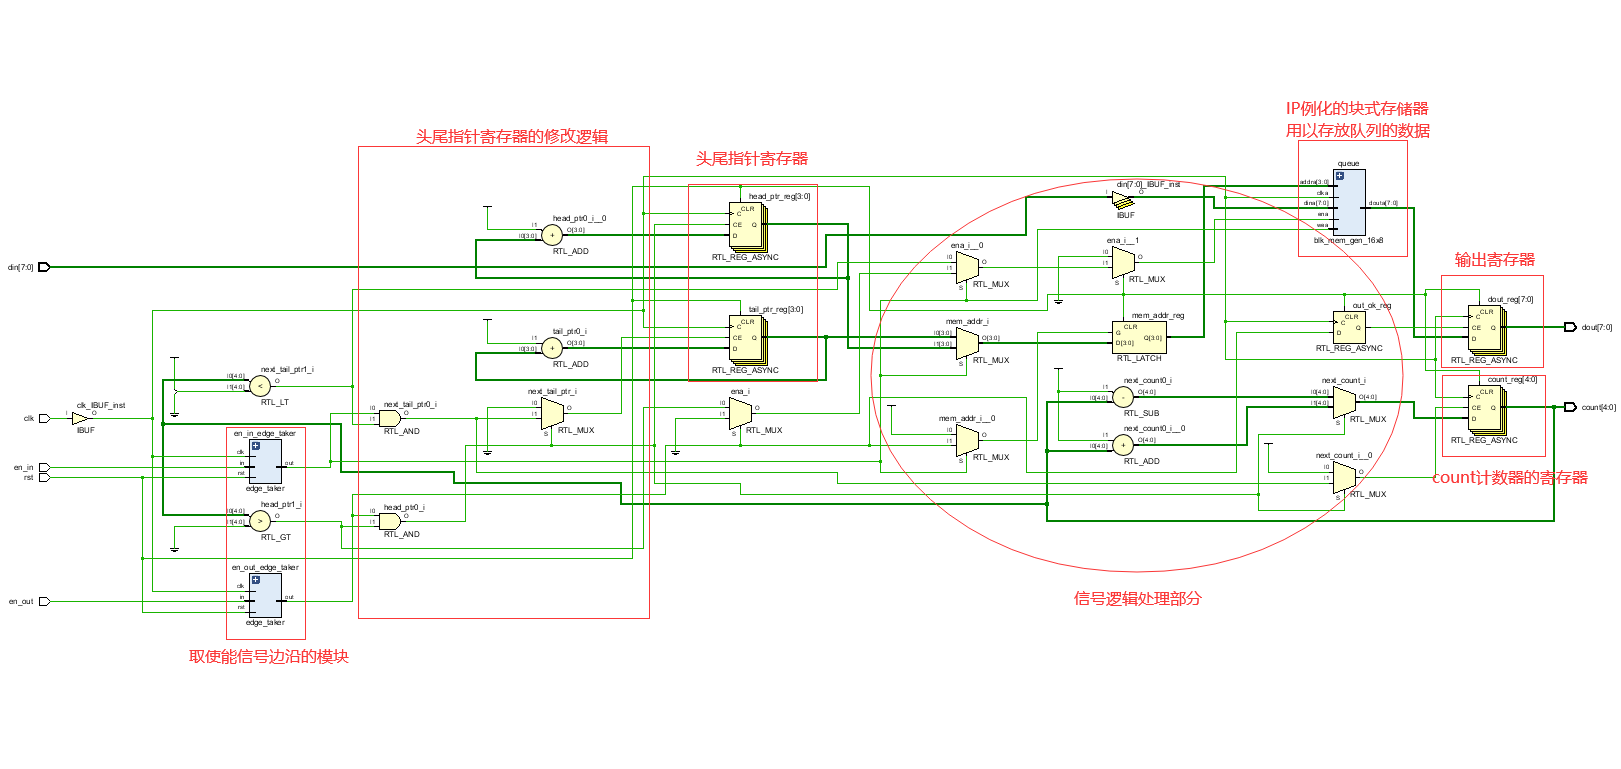
\includegraphics[scale=0.3]{data_path.png}
\end{figure}\par
\subsubsection{状态机控制}
这里状态机若画完整, 会重复很多单元, 所以只是画一个示例:
\begin{figure}[H]
	\centering
	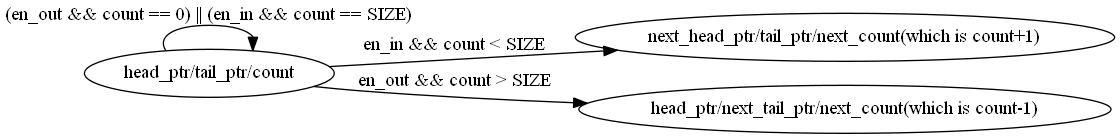
\includegraphics[scale=0.45]{graph.png}
\end{figure}\par
\subsubsection{代码讲解}
\begin{enumerate}
	\item 取边沿模块\par
	老师给出的取边沿模块略有问题, 故采用上学期模拟与数字电路实验用的取边沿模块.
	\begin{lstlisting}[language=verilog]
	module edge_taker
	    #(parameter N = 1)
	    (
	    input clk, rst, // 时钟(上升沿有效), 复位(异步复位, 高电平有效)
	    input [N-1: 0]in,   // 输入信号
	    output [N-1: 0] out   // 输出信号
	    );
	    
	    reg [N-1: 0] in1 = 0;
	    reg [N-1: 0] in2 = 0;
	    always@(posedge clk) in1 <= in;
	    always@(posedge clk) in2 <= in1;
	    assign out = rst ? {N{1'b0}} : in1 & ~in2;
	endmodule
	\end{lstlisting}
	\item FIFO队列模块\par
	代码各个部分的功能已经注释清楚. \par
	其他一些值得一提的有:
	\begin{enumerate}
		\item 如果指针到了最后一个地址, 就需要换到0地址处, 这里需要稍作处理.
		\item count会在入队时+1, 出队时-1.
		\item 当且仅当有使能信号的时候, next\_head\_ptr和next\_tail\_ptr才会是+1的状态.
		\item 其中取边沿模块可以避免一个使能信号内多次出入队列.
	\end{enumerate}
	
	\begin{lstlisting}[language=verilog]
module fifo
    #(
    parameter WIDTH = 8,
    parameter ADDR_WIDTH = 4,
    parameter SIZE = {1'b1, {ADDR_WIDTH{1'b0}}}
    )
    (
    input clk, rst,		//时钟(上升沿有效)、异步复位(高电平有效)
    input [WIDTH-1: 0] din,		//入队列数据
    input en_in, 		//入队列使能,高电平有效
    input en_out,		//出队列使能,高电平有效
    output reg [WIDTH-1: 0] dout, 	//出队列数据
    output reg [ADDR_WIDTH: 0] count	//队列数据计数
    );
    
    reg [ADDR_WIDTH-1: 0] head_ptr;
    reg [ADDR_WIDTH-1: 0] tail_ptr;
    reg [ADDR_WIDTH-1: 0] next_head_ptr;
    reg [ADDR_WIDTH-1: 0] next_tail_ptr;
    reg [ADDR_WIDTH-1: 0] mem_addr;
    reg [ADDR_WIDTH: 0] next_count;
    reg ena;
    wire [WIDTH-1: 0] mem_out;
    wire en_in_edge, en_out_edge;
    reg out_ok;
    
    // 数据通路
    //// 块内存
    blk_mem_gen_16x8 queue(.addra({mem_addr}), .clka(clk), .dina(din), .douta(mem_out), .ena(ena), .wea(en_in_edge));
    //// 取使能信号边缘
    edge_taker #(.N(1)) en_in_edge_taker(.in(en_in), .clk(clk), .rst(rst), .out(en_in_edge));
    edge_taker #(.N(1)) en_out_edge_taker(.in(en_out), .clk(clk), .rst(rst), .out(en_out_edge));
    
    // 状态机状态转移
    always @(posedge clk, posedge rst) begin
        if(rst) begin
            head_ptr <= {ADDR_WIDTH{1'b0}};
            tail_ptr <= {ADDR_WIDTH{1'b0}};
            next_head_ptr <= {ADDR_WIDTH{1'b0}};
            next_tail_ptr <= {ADDR_WIDTH{1'b0}};
            count <= {(ADDR_WIDTH+1){1'b0}};
            dout <= {WIDTH{1'b0}};
            out_ok <= 1'b0;
        end
        else begin
            head_ptr <= next_head_ptr;
            tail_ptr <= next_tail_ptr;
            count <= next_count;
            out_ok <= en_out_edge;
            if(out_ok) dout <= mem_out;
        end
    end
    
    // 状态描述
    always @(*) begin
        if(rst) begin 
            mem_addr = {ADDR_WIDTH{1'b0}};
            ena = 1'b0;
        end
        else begin
            // head\_ptr的状态控制
            if(en_out_edge && (count > 0)) begin
                next_head_ptr = head_ptr == SIZE ? 0 : head_ptr + 1;
                next_tail_ptr = tail_ptr;
                next_count = count - 1;
                mem_addr = head_ptr;
                ena = 1'b1;
            end
            // tail\_ptr的状态控制
            else if(en_in_edge && (count < SIZE)) begin
                next_head_ptr = head_ptr;
                next_tail_ptr = tail_ptr == SIZE ? 0 : tail_ptr + 1;
                next_count = count + 1;
                mem_addr = tail_ptr;
                ena = 1'b1;
            end
            else begin
                next_head_ptr = head_ptr;
                next_tail_ptr = tail_ptr;
                next_count = count;
                ena = 1'b0;
                mem_addr = mem_addr;
            end
        end
    end
    
endmodule
	\end{lstlisting}
\end{enumerate}

\section{实验结果}
\subsection{寄存器堆}
这是个简单的仿真测试. 这里寄存器刚开始读出来是x, 而后进行写入, 则异步读出的结果相应改变. 如下图.
\begin{figure}[H]
	\centering
	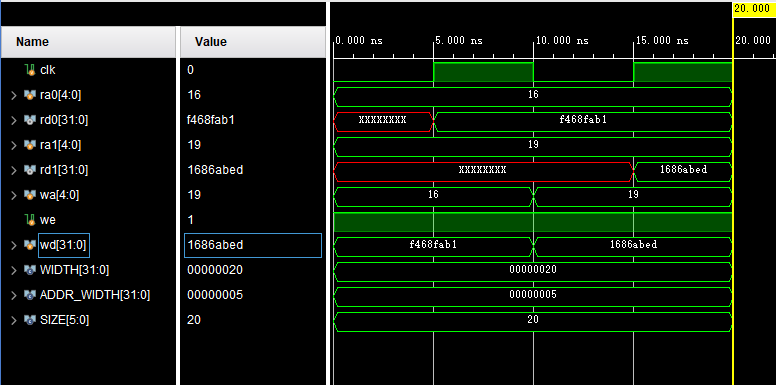
\includegraphics[scale=0.5]{register_file.png}
\end{figure}\par
因此可以认为, 该寄存器文件模块的两个异步读和一个同步写都能够正常工作.
\subsection{存储器}
该部分的实验结果已经在前面实验过程中讲述, 这里就不在重复描述了.
\subsection{FIFO队列}
下图清晰地展示了仿真过程及正确性.\par
这个仿真先后做了这些操作: push 00到0f, push ff(但由于队列大小只有2, 故失败), pop 16次(按顺序出00到0f), pop(已经没有数据, 输出不变).
此外, 图中蓝色标出了一个取边沿的示例.\par
\begin{figure}[H]
	\centering
	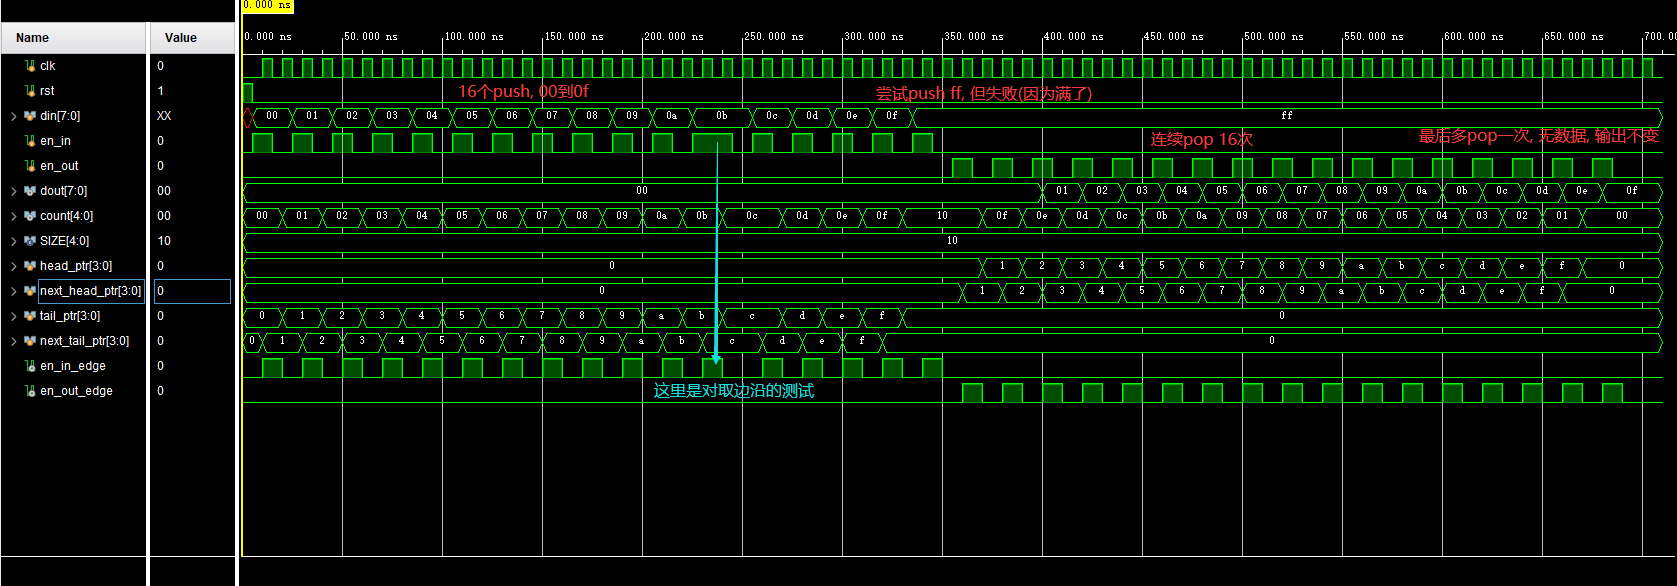
\includegraphics[scale=0.30]{queue_width4_illustrate.png}
\end{figure}\par

\section{思考题}
\subsection{如何利用寄存器堆和适当电路设计实现可变个数的数据排序电路?}
对于给定排序数据的起始地址和终止地址(这里假设顺序存储了待排数据), 可以采用冒泡排序, 两两比较和交换(类似于Lab1). 和Lab1所不同的是, Lab1的状态是程序开始前就知道的, 而这里的状态是可变的, 但此时只需要维护两个指针(类似于冒泡排序时, 两层循环分别需要的循环变量), 并依据这两个指针来控制状态转移, 即可完成可变个数的数据排序电路.

\section{心得体会}
本次实验让我更深刻地理解了 Distributed Memory 和 Block Memory 的区别, 并初次理解了怎么使用Verilog描述一个FIFO的过程.

\section{意见建议}
这次实验的FIFO的对应实验要求描述并不是特别清楚. 例如, 应当在输入之后几个周期内给出结果等. 这对我实现造成了一定困扰.

\end{document}






